\documentclass{standalone}
\usepackage{tikz}
\tikzset{   block/.style = {draw, fill=white, very thick, rectangle, minimum height=1cm, minimum width=2cm},  
            square/.style = {draw, fill=white, very thick, rectangle, minimum height=0.5cm, minimum width=0.5cm},
            sum/.style= {draw, fill=white, very thick, circle, node distance=0.5cm}}  
\begin{document}
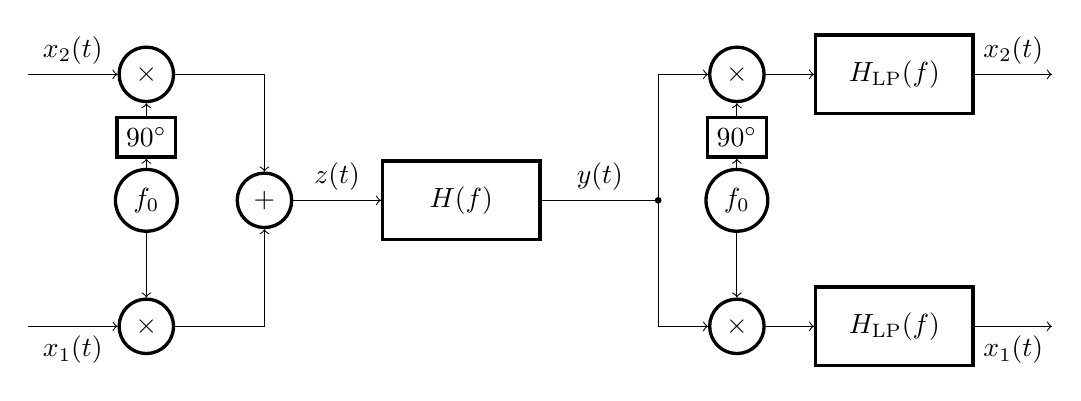
\begin{tikzpicture}[scale=2]
    \node[sum](s1)at(0.25,0.8){$\times$};
    \node[sum](s2)at(0.25,-0.8){$\times$};
    \draw[->](-0.5,0.8)--(s1.180)node[midway, above]{$x_2(t)$};
    \draw[->](-0.5,-0.8)--(s2.180)node[midway, below]{$x_1(t)$};
    \node[sum](o1)at(0.25,0){$f_0$};
    \node[square](f1)at(0.25,0.4){$90^{\circ}$};
    \draw[->](o1.90)--(f1.270);
    \draw[->](f1.90)--(s1.270);
    \draw[->](o1.270)--(s2.90);

    \node[sum](s3)at(1,0){$+$};
    \draw[->](s1.0)--(1,0.8)--(s3.90);
    \draw[->](s2.0)--(1,-0.8)--(s3.270);
    \node[block](h)at(2.25,0){$H(f)$};
    \draw[->](s3.0)--(h.180)node[midway, above]{$z(t)$};
    \draw[-](h.0)--(3.5,0)node[midway, above]{$y(t)$};
    \filldraw[black](3.5,0)circle(0.5pt);
    \node[sum](s1)at(4,0.8){$\times$};
    \node[sum](s2)at(4,-0.8){$\times$};
    \draw[->](3.5,0)--(3.5,0.8)--(s1.180);
    \draw[->](3.5,0)--(3.5,-0.8)--(s2.180);
    \node[sum](o1)at(4,0){$f_0$}; 
    \node[square](f1)at(4,0.4){$90^{\circ}$};
    \draw[->](o1.90)--(f1.270);
    \draw[->](f1.90)--(s1.270);
    \draw[->](o1.270)--(s2.90);

    \node[block](b1)at(5,0.8){$H_\mathrm{LP}(f)$};
    \node[block](b2)at(5,-0.8){$H_\mathrm{LP}(f)$};
    \draw[->](s1.0)--(b1.180);
    \draw[->](s2.0)--(b2.180);
    \draw[->](b1.0)--(6,0.8)node[midway, above]{$x_2(t)$};
    \draw[->](b2.0)--(6,-0.8)node[midway, below]{$x_1(t)$};
\end{tikzpicture}
\end{document}